\begin{center}
	\section{An\'alisis de resultados}
\end{center}

\noindent
\justify

La simulaci\'on num\'erica CFD, desarrollada con el solucionador \texttt{pimpleFoam}, de OpenFOAM, encontr\'o su punto de equilibrio (punto \textit{estacionario}) al cabo de ocho segundos de simulaci\'on. En la Figura \ref{CFD:vel} se observa un valor de velocidad m\'axima de $0.0018 [m/s]$ que es alcanzado en la primera lamela y decrece en las lamelas consecuentes hasta un valor cercano de $0.0012 [m/s]$; fen\'omeno f\'isico que va acorde a la realidad por tratarse de flujos en serie.

\noindent
\justify

En la Figura \ref{CFD:p} se puede apreciar el perfil de presiones sobre el sistema; en donde se presenta un comportamiento uniforme y sim\'etrico alcanzando un valor de presi\'on m\'axima de hasta $5.90 \cdot 10^{-6} [kPa]$. Como era de esperarse, las condiciones de frontera establecidas en la secci\'on \ref{CondF} fueron respetadas: en la salida del flujo se aprecia una presi\'on manom\'etrica de $0 [KPa]$ (atmosf\'erica) y la velocidad de flujo en la entrada es de $0.00097 [m/s] \approx 3.493 [m/h]$.

\noindent
\justify

Comparando las Figuras \ref{CFD:vel} y \ref{CFDEM:vel}, se puede apreciar c\'omo el solvente cambia la distribuci\'on de velocidades por la sedimentaci\'on sufrida por las part\'iculas de arena, cuya densidad es mayor que la del fluido circundante; raz\'on por la que el solvente tiende a moverse con mayor velocidad en las \'ultimas lamelas en lugar de las primeras, a diferencia de lo observado en la secci\'on \ref{CFD:resultados}. Debido a ello, es posible clasificar a las lamelas por zonas de \textit{``pureza"} durante el proceso de separaci\'on: en donde las primeras cuatro presentan menor concentrac\'on particular que las \'ultimas cuatro.

\noindent
\justify

La presencia de v\'ortices y remolinos en la simulaci\'on CFD-DEM rectifica la decisi\'on de haber empleado un solucionador basado en \texttt{pimpleFoam}, el cual fue adaptado para resolver el problema \textit{Euler - Lagrange} (E - L).

\noindent
\justify

Diferente al fen\'omeno apreciado en la Figura \ref{CFD:p}, la distribuci\'on de presiones en la Figura \ref{CFDEM:p} no es sim\'etrica y tiende a presentar sus m\'aximos valores en la zona de congregaci\'on de los sedimentos.

\begin{figure}[h!]
	\centering
	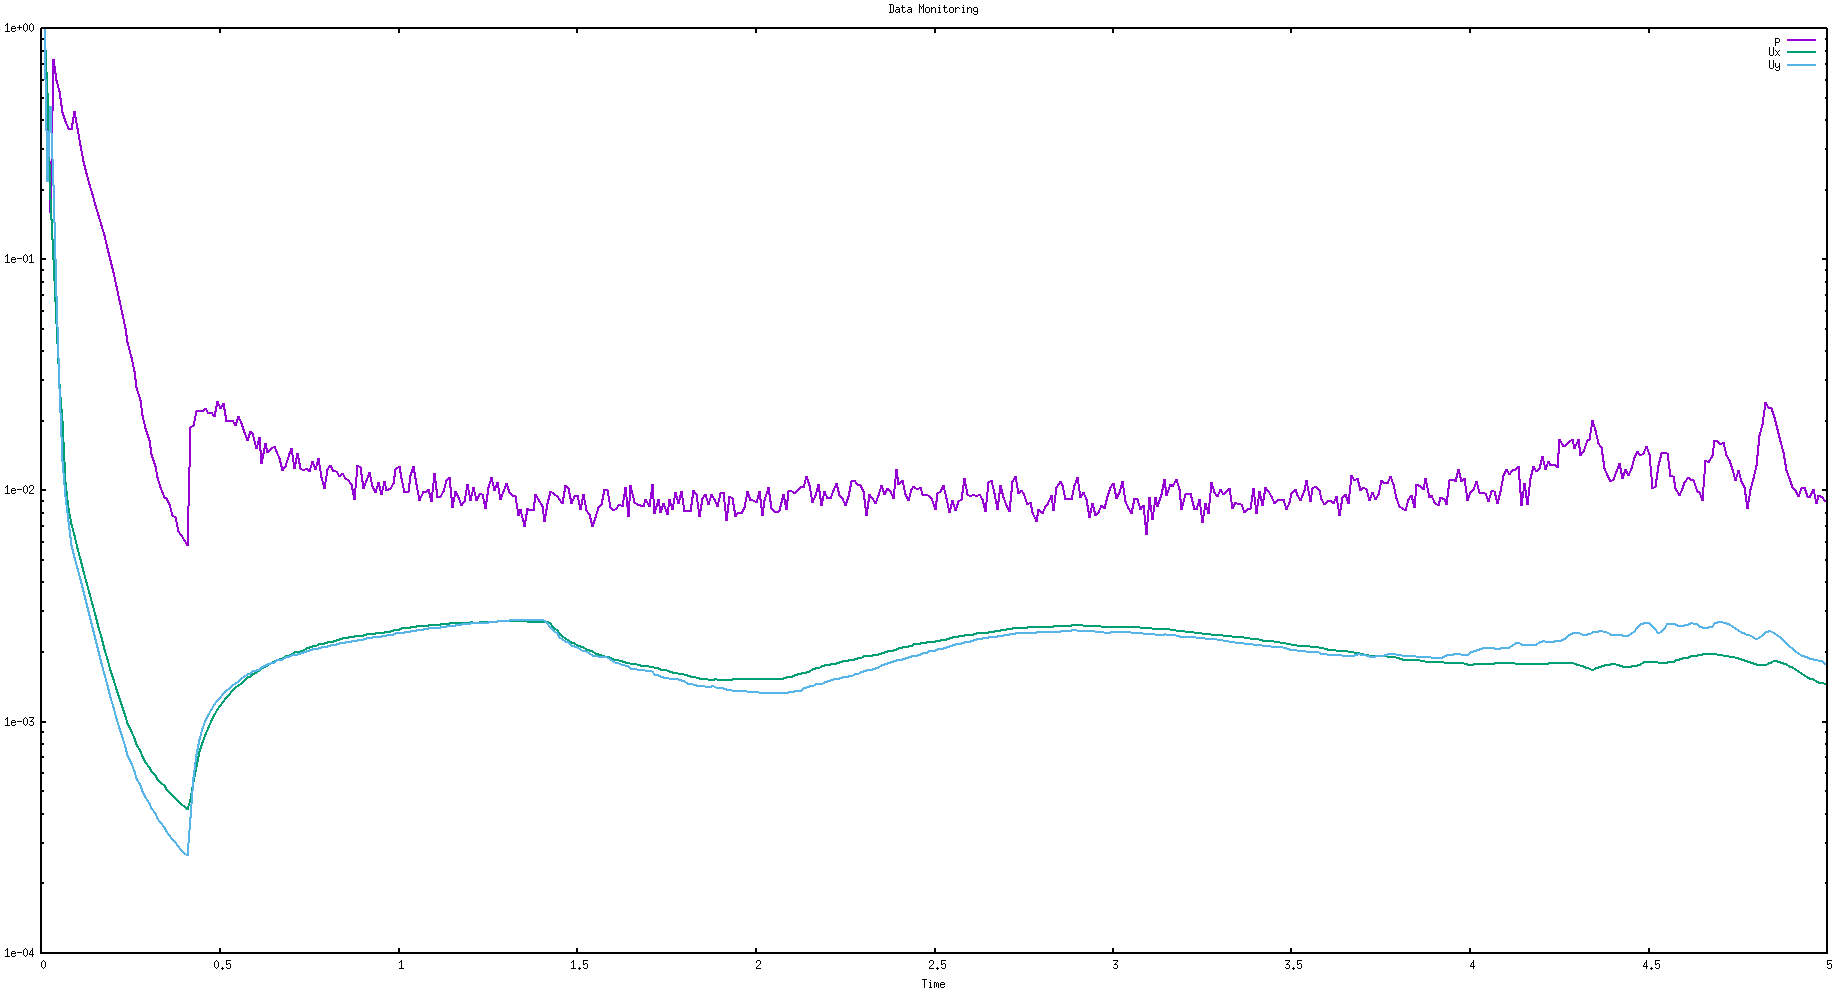
\includegraphics[width=\textwidth]{Images/CFDEM/residuals.png}
	\caption{Monitoreo de residuales en la simulaci\'on CFD-DEM.}
	\label{CFDEM:residuals}
\end{figure}

\noindent
\justify

De la Figura \ref{CFDEM:residuals}, la l\'inea morada corresponde al residual de la presi\'on, la de color cian al residual de la velocidad en $y$ y la de color verde al residual de la velocidad en $x$. El comportamiento de los residuales est\'a directamente relacionado con la magnitud de los errores en la soluci\'on de las ecuaciones gobernantes$^{\cite{Liang2018}}$. 

\newpage

\noindent
\justify

Debido al hecho de que los residuales tienden a aglomerarse en valores cercanos a cero, son un indicativo de alta precisi\'on del modelo num\'erico implementado. Las variaciones vistas en los residuales de presi\'on se deben a la vorticidad originada por los reflujos consecuentes a la interacci\'on fluido - part\'icula. Durante la simulaci\'on, se observ\'o una estabilizaci\'on en los perfiles de velocidad; raz\'on por la que los residuales $U_x$ y $U_y$ presentan un comportamiento sin fluctuaciones y con peque\~nas variaciones durante el desarrollo del flujo dentro del volumen de control.